\documentclass[ngerman]{scrartcl}

\KOMAoptions{fontsize=11pt,paper=a4}
\KOMAoptions{DIV=14}

\usepackage{babel}
\usepackage[utf8]{inputenc}
\usepackage[T1]{fontenc}
\usepackage[autostyle=true]{csquotes}
\usepackage{amsmath}
\usepackage[varg]{txfonts}
\usepackage{graphicx}
\usepackage{hyperref}

\graphicspath{{figs/}}

\begin{document}

\title{Übungsblatt 1 zur Vorlesung 'Numerische Methoden der Physik' SS 2015}
\subtitle{Madelung-Energie des NaCl-Kristalls}
\author{Fabian Schmidt und Marvin Schmitz}
\maketitle

\newpage

\section*{Physikalische Beschreibung des Problems}
Wir betrachten einen Kochsalz-Kristall bestehend aus Natrium- (Na) und Chlorid-Ionen (Cl).
In einem NaCl-Kristallgitter sind Na+ und Cl- Ionen aufgrund ihrer Ladung durch die Coulomb-Kraft gebunden.
In dieser Arbeit wollen wir nun die Bindungsenergie $V$ eines einzelnen Ions im Kristallgitter numerisch bestimmen.\\

Die Bindungsenergie $V_{ij}$ zweier Ladungen $e_i$, $e_j$ im Abstand $r$ beträgt
\begin{align*}
	V_{ij} = \frac{1}{4\pi \epsilon_0} \cdot \frac{e_ie_j}{r_{ij}}.
\end{align*}

In einem NaCl-Kristall sind die Ionen kubisch angeordnet, so dass der Abstand $r_{ij}$ zweier Ionen $i$,$j$ am Ort 
$i = (i_1,i_2,i_3)$ und $j = (j_1,j_2,j_3)$ gegeben ist durch
\begin{align*}
	r_{i,j} = a\cdot \sqrt{(i_1-j_1)^2+(i_2-j_2)^2+(i_3-j_3)^2},
\end{align*}
mit der Gitterkonstanten $a$.\\

Wir betrachten nun im Folgenden das Ion am Ort $j = (0,0,0)$.
Die Ladung der Kationen (Na+) und Anionen (Cl-) ist die positive/negative Elementarladung $e$.
Da sich die Na+/Cl-Ionen im Kristall jeweils abwechseln, folgt für die Bindungsenergie $V_{ij}$
zwischen dem Ion am Ort $j$ und einem weiteren Ion am Ort $i = (i,j,k)$:
\begin{align*}
	V_{ij} = \frac{1}{4\pi \epsilon_0} \cdot \frac{e^2}{a} \frac{(-1)^{i+j+k}}{\sqrt{i^2+j^2+k^2}}.
\end{align*}

Die gesamte Bindungsenergie $V$ eines einzelnen Ions erhalten wir nun durch Summation der Energien $V_{ij}$
für alle Ionen eines Kristalls. Diese Energie ist die Madelungenergie.
Die Madelung-Konstante ist definiert durch diese Summe, jedoch ohne die konstanten Vorfaktoren.

\section*{Modellierung des Problems}
Ein NaCl-Kristall (kubisches Kristallgitter) bildet makroskopisch die Struktur eines Quaders aus (siehe Abbildung 1).
%\begin{figure}[Text]
%\centering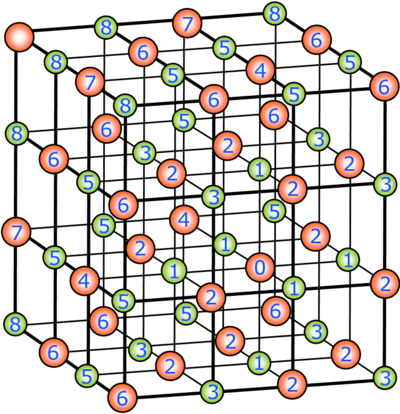
\includegraphics[width=9cm]{madelung}
%\end{figure}
Aus diesem Grund summieren wir über einen Würfel der Kantenlänge $n$, so dass $i$,$j$,$k$ von $-n$ bis $n$ laufen.\\
Um einen elektrisch neutralen Kristall zu erhalten, berücksichtigen wir, dass die Ionen auf dem aüßersten Rand
des Würfels nur Teilladungen besitzen. Diese betragen $ 1/8 $ an den Ecken, $ 1/4 $ an den Kanten und $ 1/2 $ auf der Fläche.

%TODO:Desweiteren betrachten wir zusätzlich nochmal den Fall eines flachen Kristallgitters also $i_3=j_3$.


\section*{Implementierung der Lösung}
Wir berechnen mit einer Funktion madelung2d(int n)  bzw. madelung3(int n) die Madelung-Konstante eines Würfels der Kantenlänge $n$.
Dazu wird in drei verschachtelten Schleifen über die Koordinaten $i$,$j$,$k$ iteriert. Innerhalb der Schleife wird unterschieden,
ob sich das jeweilige Ion am Ort $(i,j,k)$ auf dem Rand befindet order nicht.
Die Beiträge dieser Ionen werden dann mit den oben diskutierten Faktoren gewichtet.\\

Die Funktion bindungsenergie(dim,d,var) berechnet nun für einen NaCl-Kristall mit Gitterkonstante $d$ die Madelungenergie mit einer Genauigkeit vom $var$.
Ihr übergeben wir mit dim die Dimension (2/3), welche entscheidet, ob die Madelung-Konstante
mit madelung2d oder madelung3d berechnet wird.
Die Genauigkeit wird mittels einer while-Schleife und dem Parameter var bestimmt. Die gewünschte Genauigkeit ist erreicht, wenn die Bindungsenergie in einem Kristall der Kantenlänge $n$ geteilt durch die Energie in einem Kristall der Kantenlänge $n-1$ kleiner eins ist.\\

Ist die Madelungkonstante hinreichend genau bestimmt, so wird sie mit den entsprechenden Vorfaktoren multipliziert und dieser Wert zurückgegeben.
Die main-Funktion ruft nun zweimal bindungsenergie() auf, um die Madelung-Energie eines 2-/3-dimensionalen Kristalls zu berechnen und
gibt den entsprechenden Wer auf der Konsole aus.

Um den Term $(-1)^{n}$ schneller zu berechnen, wurde die Funktion powm1(n) implementiert. Sie nutzt aus, dass man von n nur wissen muss,
ob n gerade oder ungerade ist.
\section*{Ergebnis}
Unser Programm ermittelt für einen 2D-Kristall und eine Genauigkeit von $10^{-5}$ die Madelungenergie zu
\begin{align*}
	E_{2D} = 6.631798 \cdot 10^{-19} J
\end{align*}
und für einen dreidimensionalen Kristall der Kantenlänge $n = $
\begin{align*}
	E_{3D} = 7.193871E-19 J.
\end{align*}
Leider dauert die Berechnung für 3D sehr lange, wenn die gewünschte Genauigkeit größer als $10^{-2}$ ist.

\section*{Ausblick}
Um die Berechnung zu optimieren, kann die Evjen-Methode eingesetzt werden. Dabei wird das mittlere Ion
eines Würfels der Kantenlänge $2n+1$ betrachtet. Nun iteriert man nicht mehr über alle anderen Ionen,
sondern nurnoch die Ionen eines Oktanten, d.h. die Anzahl der Schritte verringert sich um einen Faktor $1/8$.
Dabei ist zu beachten, dass die Ionen auf den Achsenflächen nur mit einem entsprechenden Faktor $1/2$,$1/4$ und $1/8$
einfliessen dürfen, da auch hier der Kristall elektrisch neutral bleiben soll.

\end{document}
